\section{Durchführung}

In dem Experiment wird der in Abbildung \ref{fig:aufbau} dargestellte Aufbau
verwendet.

\begin{figure}[H]
  \centering
  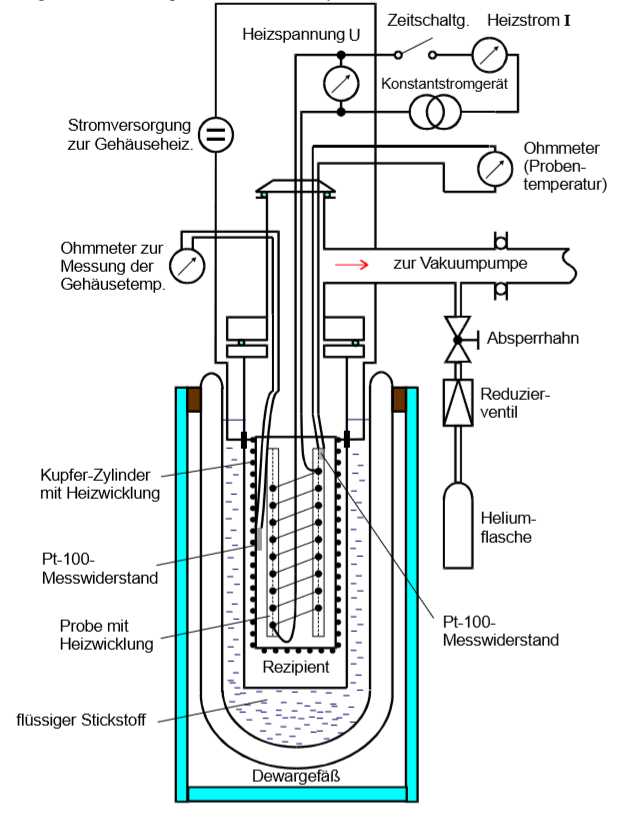
\includegraphics[width=10cm]{aufbau.png}
  \caption{In dem Experiment verwendeter Aufbau \cite{skript}}
  \label{fig:aufbau}
\end{figure}

Zu Beginn der Messung wird der Rezipient evakuiert und dann mit Helium gefüllt.
Das Dewar-Gefäß, das den Rezipienten umgibt, wird dann mit flüssigem
Stickstoff gefüllt, damit der Rezipient die Temperatur von dem Stickstoff, also
ungefähr $\SI{80}{\kelvin}$, annimmt. Es dauert ungefähr eine Stunde,bis
die Probe ungefähr auf diese Temperatur abgekühlt ist. Danach wird der Rezipient erneut evakuiert,
um Wärmeverlust durch Konvektion zu vermeiden. Die kalte Probe im Rezipienten
wird dann mit Hilfe einer Heizwicklung erwärmt, ihr wird also elektrische
Energie zugeführt. Zur Messung der Temperatur wird ein Thermowiderstand verwendet.

Energieverluste können in diesem Versuch nicht nur durch Konvektion, also
den Wärmeverlust durch Teilchenströme, entstehen. Ein weiterer Energieverlust
ist durch Wärmestrahlung gegeben. Wird die Probe erhitzt, so strahlt sie
Wärme ab. Um diese Verluste zu minimieren, wird der Kupfer-Zylinder mit
Heizwicklung auf die Temperatur der Probe geregelt. Dadurch strahlt
auch die Heizwicklung Wärme ab, welche von der Probe wieder aufgenommen wird.
Dadurch sollte bei optimaler Abstimmung der Wärmeverlust durch Wärmestrahlung
verringert werden.
